\documentclass[12pt, letterpaper, twoside]{article}
\usepackage{nopageno,epsfig, amsmath, amssymb}
\usepackage{physics}
\usepackage{mathtools}
\usepackage{hyperref}
\usepackage{xcolor}

\usepackage[letterpaper,
            margin=0.8in]{geometry}

\title{Astro 519A; Problem Set 3}
\author{\textbf{Tom Wagg}}

\newcommand{\answer}[1]{
    \par\noindent\rule{\textwidth}{0.4pt}\\#1\\
}

% custom function for adding units
\makeatletter
\newcommand{\unit}[1]{%
    \,\mathrm{#1}\checknextarg}
\newcommand{\checknextarg}{\@ifnextchar\bgroup{\gobblenextarg}{}}
\newcommand{\gobblenextarg}[1]{\,\mathrm{#1}\@ifnextchar\bgroup{\gobblenextarg}{}}
\makeatother

\newcommand{\avg}[1]{\left\langle #1 \right\rangle}
\allowdisplaybreaks

\begin{document}

\maketitle

{\it \noindent 1). {\it [11/2 class]} quick special relativity questions\\
a) At what speed does a clock move if it runs at a rate which is one-half the rate of a clock at rest?}

\answer{
    \begin{align}
        t &= t_0 \gamma \\
        \gamma &= 2 \\
        \Aboxed{ v &= \sqrt{3}/2 c = 0.87 c }
    \end{align}
}

{\it \noindent b) At what speed does a meter stick move if its length is observed to shrink to 0.5 m?}

\answer{
    \begin{align}
        L &= \frac{L_0}{\gamma} \\
        \gamma &= 2 \\
        \Aboxed{ v &= \sqrt{3}/2 c = 0.87 c }
    \end{align}
}

{\it \noindent c) The average lifetime of a $\pi$ meson in its own frame of reference is 26.0 ns. (This is its proper lifetime.) If the $\pi$ meson moves with speed $0.95c$ with respect to the Earth, what is its lifetime as measured by an observer at rest on Earth? What is the average distance it travels before decaying as measured by an observer at rest on Earth?}

\answer{
    \begin{align}
        t &= \gamma t_0 \\
        &= \frac{26 \times 10^{-9} \unit{s}}{\sqrt{1 - 0.95^2}} \\
        \Aboxed{ t &= 8.3 \times 10^{-8} \unit{s} } \\
        d &= v t \\
        &= 0.95 c \cdot 8.3 \times 10^{-8} \unit{s} \\
        \Aboxed{ d &= 24 \unit{m} }
    \end{align}
}

{\it \noindent d) An atomic clock is placed in a jet airplane. The clock measures a time interval of 3600 s when the jet moves with speed 400 m/s. How much longer or shorter a time interval does an identical clock held by an observer on the ground measure?}

\answer{
    This seems like a trick question upon first reading since we are told ``the clock measures'' its time on the plane, not that a stationary observer measures the clock. But assuming it is not a trick question then we find that the time measured on the ground would be longer by a factor
    \begin{equation}
        \boxed{ \gamma = \qty(1 - (400 \unit{m}{s^{-1}}) / c^2)^{-1/2} = 1.0000000000009 }
    \end{equation}
}

{\it 2) {\it [11/4 class]} A massive space fleet of hostile aliens is traveling towards the Earth.  
 
a.) The aliens' ``hyperdrive'' operates at a Lorentz factor of $\gamma=100$.  Still, traveling 100 light years -- the distance from their home planet to the earth in the CMB rest frame -- takes a long time!  How much time passes for the aliens on the ship?  Assume that the time it takes to accelerate to $\gamma=100$ and then back down is small such that most of the trip is spent at $\gamma=100$.}

\answer{
    Since we are in the frame of the aliens on the ship, we just need to find their velocity and divide the distance by it. Since $\gamma$ is so high, the speed of the aliens is going to be extremely close to the speed of light and so we can simply state the time that would pass, given the definition of a light year, would be simply
    \begin{equation}
        t = 100 \unit{years}
    \end{equation}
    And in the alien's frame this would be
    \begin{equation}
        \boxed{ t = 1 \unit{year} }
    \end{equation}
}

{\it b.) In their frame and halfway between the solar system and their home planet, they broadcast isotropically a signal with average bolometric power $P$.  What is the average bolometric flux ($F =\int d\nu F_\nu$) received at both locations?}

\answer{
    We can apply Eq. 4.97b from RL for this problem
    \begin{equation}
        \dv{P_r}{\Omega} = \frac{1}{\gamma^4 (1 - \beta \mu)^4} \dv{P}{\Omega},
    \end{equation}
    where $P_r$ is the received power and $\mu$ is the dependent on the angle such that $\mu = 1$ in the forward direction and $\mu = -1$ in the backward direction. We can write the flux received at both locations as
    \begin{align}
        F &= \dv{P_r}{A} \\
        &= \dv{P_r}{\Omega} \dv{\Omega}{A} \\
        &= \dv{P_r}{\Omega} \frac{1}{(50 \unit{lyr})^2} \\
        F &= \frac{1}{\gamma^4 (1 - \beta \mu)^4} \frac{P}{4 \pi} \frac{1}{(50 \unit{lyr})^2}
    \end{align}
    So now it's just a matter of evaluating! Note that $\beta = \sqrt{1 - 10^{-4}}$ (from rearranging $\gamma = 100$). For the forward direction we have $\mu = 1$ and thus
    \begin{equation}
        \boxed{ F_{\rm sol} = \frac{1}{\gamma^4 (1 - \beta)^4} \frac{P}{4 \pi} \frac{1}{(50 \unit{lyr})^2} = 5.7 P \times 10^{-32} \unit{cm^{-2}} }
    \end{equation}
    and for the backward direction $\mu = -1$ and we get
    \begin{equation}
        \boxed{ F_{\rm alien} = \frac{1}{\gamma^4 (1 + \beta)^4} \frac{P}{4 \pi} \frac{1}{(50 \unit{lyr})^2} = 2.2 P \times 10^{-50} \unit{cm^{-2}} }
    \end{equation}
    Thus we find that the flux in the forward direction is approximately $2.6 \times 10^{18}$ times stronger in the backward direction, oh my!
}

{\it c.)  On the way, their ship hits large dust particles with diameter $D = 1\mu m$ and density $\rho = 1$gr/cm$^3$. What is the energy in each impact?  Compare to the energy of a 10kg bowling ball moving at $36~$km/hr.}

\answer{
    We can take that the relative Lorentz factor between the dust particle and the ship is $\gamma = 100$. Thus the kinetic energy that is absorbed during each impact is
    \begin{equation}
        E = (\gamma - 1) m c^2,
    \end{equation}
    where the minus one is because the rest mass of the particle stays behind (though this factor makes almost no different the final result). Next we just need to solve for the mass using the radius and density
    \begin{equation}
        m = \rho V = \frac{4 \pi r^3 \rho}{3} = 5.24 \times 10^{-12} \unit{kg}
    \end{equation}
    Plugging this all in we find that the energy of each impact is
    \begin{equation}
        \boxed{ E_{\rm grain} = 99 \cdot 5.24 \times 10^{-12} \cdot (3 \times 10^8)^2 \unit{J} = 4.7 \times 10^{10} \unit{erg} }
    \end{equation}
    The kinetic energy of the bowling ball would be
    \begin{equation}
        \boxed{ E_{\rm ball } = \frac{1}{2} m v^2 = 5 \times 10^9 \unit{erg} }
    \end{equation}
    and so the bowling ball has a factor of 10 lower energy than the dust grains.
}

{\it d) The ``reddening'' of these dust grains is such that they absorb $10\%$ of background optical light towards this star. Estimate the average number density of dust grains along the path by assuming that they have a geometric cross section of $\pi (D/2)^2$, valid for $\lambda \lesssim D$.  What is the flux of impacts hitting the ship? (Answer in the Earth's frame.) }

\answer{
    We are told that $10\%$ of light is absorbed by the dust grains and thus we know that
    \begin{equation}
        e^{-\tau} = 0.9,
    \end{equation}
    where $\tau$ is the optical depth. From the definition of the optical depth we can then solve for the for the number density
    \begin{align}
        \tau &= \int n \sigma \dd{s} \\
        \ln \frac{10}{9} &= n \sigma s \\
        \ln \frac{10}{9} &= n \pi \qty(\frac{D}{2})^2 s \\
        n &= \frac{1}{\pi} \ln \frac{10}{9} \qty(\frac{2}{D})^2 \frac{1}{s} \\
        &= \frac{1}{\pi} \ln \frac{10}{9} \qty(\frac{2}{\unit{\mu m}})^2 \frac{2}{100 \unit{lyr}} \\
        \Aboxed{ n &= 2.8 \times 10^{-13} \unit{cm^{-3}} }
    \end{align}
    The flux of impacts hitting the ship can be found as follows
    \begin{align}
        F &= \frac{N}{A t} = \frac{n V}{A t} = \frac{n d}{t} = n v \\
        \Aboxed{ F &= 0.008 \unit{cm^{-2}}{s^{-1}} }
    \end{align}
}

{\it 3) {\it [11/9 class]} free-free. 
Fast radio bursts indicate that the light travels through an electron column that is quite large with $\int n(s) ds \sim 1000$pc~cm$^{-3}$, which is measured by using that the group velocity of radio waves is slower than the speed of light in a plasma with a known frequency dependence. If FRBs were cosmological, which we now know is the case, such an electron column would arise if the come from a redshift of $z\sim 1$.  For this reason, there was intense interest in the FRB phenomena. HII regions can span a huge range of hydrogen densities, from $10-10^6$cm$^{-3}$, and have temperatures of $10^4$K. Another idea was that they were radio bursts from stars, where the electron column comes from within a radius of the star, near the stellar photosphere. The conditions then would be that the column originates from within $\lesssim 1 R_\odot$, i.e. within a solar radius, and the temperature is likely a coronal temperature of $T\sim 10^6$K.\\

a) Assume Solar metallicity. (i) At what fractional accuracy does the metallicity of the star/HII region matter for computing the free-free optical depth?   It's fine to consider just oxygen, which is the most abundant metal, and note that oxygen is a part in a thousand the hydrogen number abundance at Solar metallicity. (ii) How important is the free-free off of helium ions, which comprise 10\% of the total number density of ions?}

\answer{
    From RL Eq. 5.18a we can surmise that
    \begin{equation}
        \alpha^{\rm ff} \propto Z^2 n_i,
    \end{equation}
    and we additionally know that $\tau \propto \alpha$ and so
    \begin{equation}
        \tau^{\rm ff} \propto Z^2 n_i.
    \end{equation}
    For hydrogen, $Z = 1$ and $n_i = n_H$ and we will use this to compare. For the first part of the question, we have that $Z = 8$ and $n_i = n_O = n_H / 1000$. Therefore the fractional accuracy at which metallicity matters is
    \begin{equation}
        \boxed{ {\rm fractional\ accuracy} = \frac{8^2}{1000} = 0.064 }
    \end{equation}
    For the helium we have that $Z = 2$ and $n_i = n_{He} = n_H / 10$. Thus we can write
    \begin{equation}
        \boxed{ {\rm fractional\ accuracy} = \frac{2^2}{10} = 0.4 }
    \end{equation}
}

{\it b) One question the community asked was whether free-free absorption would absorb the FRB in some of these cases, where the observations were all at $\sim 1$GHz. Comment on whether some or all of the HII region and flaring star scenarios would be ruled out by free free absorption from the host nebulae absorbing the flux from the FRB.  Consider the range of densities for the HII region scenario and distances from the stellar surface for the star scenario given above.}

\answer{
    We can answer this question by comparing the optical depth in each case to $\tau = 1$. We can find the optical depth as
    \begin{equation}
        \tau = N \sigma = N \alpha / n,
    \end{equation}
    where $N$ is the column density and the absorption coefficient is found using RL Eq. 5.19b
    \begin{equation}
        \alpha = \frac{4 e^6}{3 m k_B c} \qty(\frac{2 \pi}{3 k_B m})^{1/2} T^{-3/2} Z^2 n_e n_i \nu^{-2} \tilde{g}_{\rm ff}.
    \end{equation}
    So we can combine these to writ ethat the optical depth is
    \begin{equation}
        \tau = \qty(0.018 \unit{cm^5}{K^{3/2}}{s^{-2}}) T^{-3/2} \nu^{-2} N n
    \end{equation}
    Let's first just consider the HII region scenario. In this case, we have that
    \begin{align}
        \tau_{\rm HII} &= \qty(0.018 \unit{cm^5}{K^{3/2}}{s^{-2}}) (10^4 \unit{K})^{-3/2} (1 \unit{GHz})^{-2} (1000 \unit{pc}{cm^{-3}}) \\
        \Aboxed{ \tau_{\rm HII} &= 5.5 n \times 10^{-5} \unit{cm^{3}} }
    \end{align}
    where we have assumed that for an HII region, $Z = 1$ and $n = n_e = n_i$ and that the Gaunt factor is approximately 1. Thus we can see that over the range of densities in an HII region ($n = 10$ to $n = 10^6$), for most densities the optical depth will be much less than 1 but for the higher density regions some and eventually all of the FRBs can be absorbed. In particular, at $n = 18000 \unit{cm^{-3}}$, the optical depth would be equal to 1.
    
    And also because I really have nothing better to be doing with my time I also made a quick plot of how the fraction absorbed changes as a function of number density. You can see in the plot that once the number density is around $2000 \unit{cm^{-3}}$ then 10\% will get absorbed and once it hits $10^5 \unit{cm^{-3}}$ pretty much everything will get absorbed. Fun :D
    
    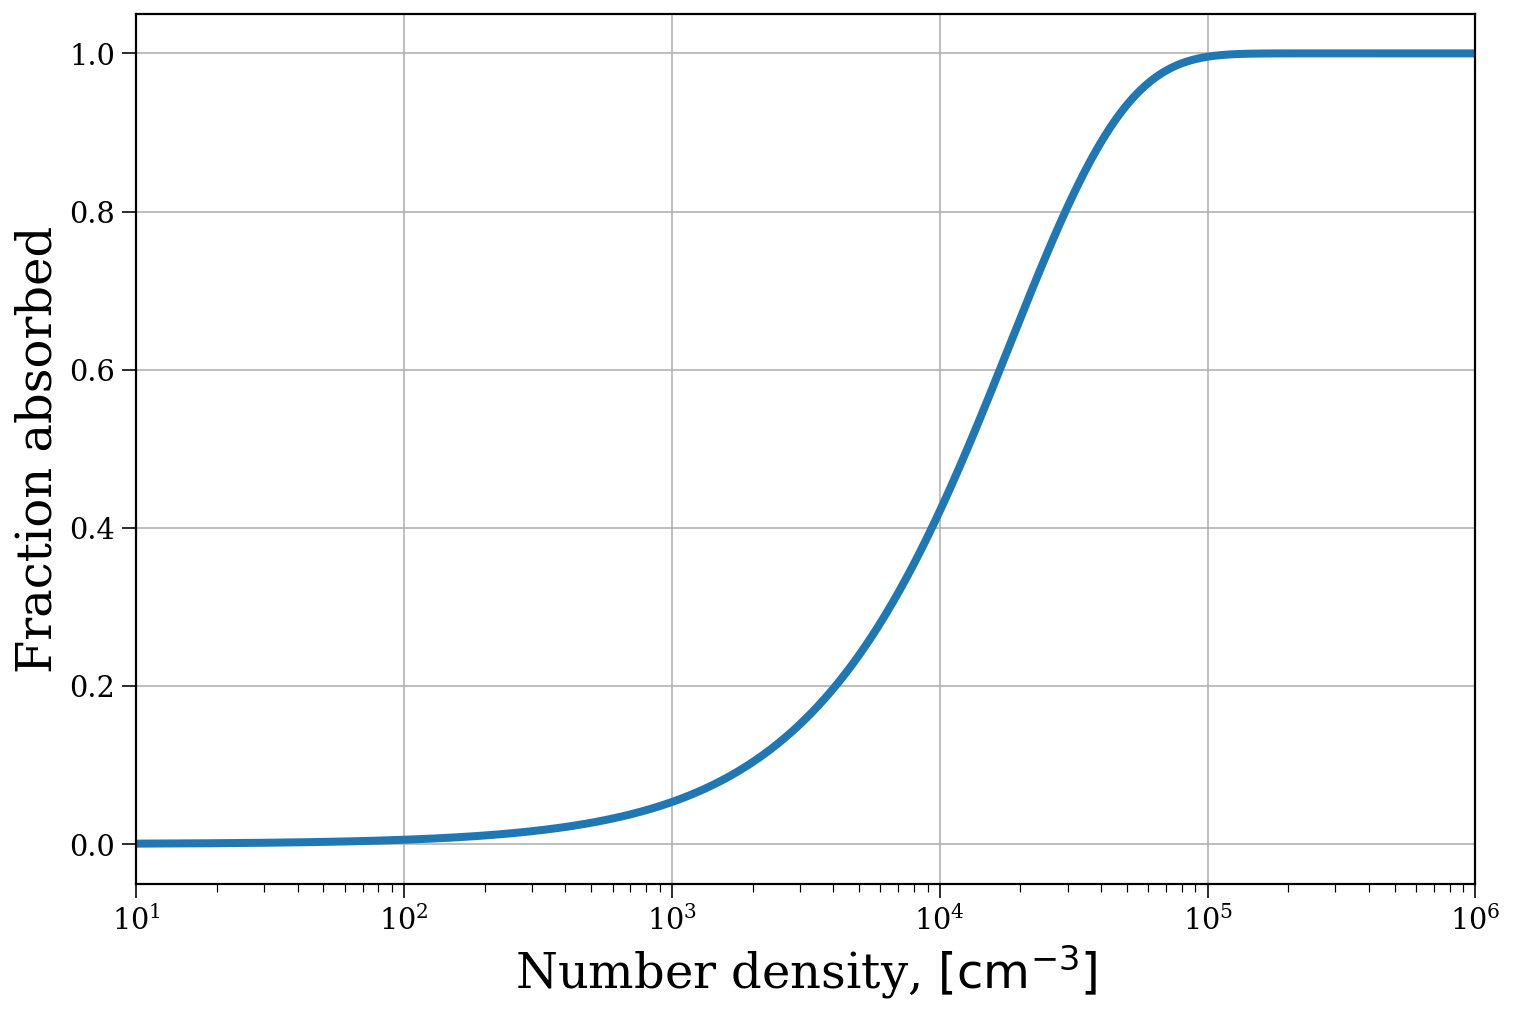
\includegraphics[width=\textwidth]{figures/astro519_ps3_q3b.png}
    
    Now let's consider the other case. The one small addition is that we need to find the number density by dividing the column density by the distance
    \begin{equation}
        n_{\rm flare} = \frac{N}{s} = \frac{N}{R_\odot}
    \end{equation}
    And with that we can immediately write down the absorption coefficient and optical depth
    \begin{align}
        \tau_{\rm flare} &= \qty(0.018 \unit{cm^5}{K^{3/2}}{s^{-2}}) (10^6 \unit{K})^{-3/2} \qty(\frac{N^2}{R_\odot}) (1 \unit{GHz})^{-2} \\
        \Aboxed{ \tau_{\rm flare} &= 2425 }
    \end{align}
    And thus we see that this optical depth is \textit{wayyy} above one and so everything is absorbed.
}

{\it c) Young neutron stars -- what likely produce FRBs -- often inhabit a bubble of electron-positron pairs.  Could a dense electron-positron pair plasma with temperature $10^{10}$K contribute substantial free-free absorption?}

Yup! Given the dipole approximation, a dense collection of pairs of positive and negative charges will contribute substantial free-free absorption. Assuming that the density is high enough and given that the temperature is particularly high, I imagine this would cause substantial absorption. Some caveats to this are that I'm not sure if the dipole approximation holds because the positive charge will move a lot (unlike in ions) and that I am assuming that there is no annihilation.

{\it 4.) {\it [11/11 class]}  Synchrotron and inverse Compton.\\
Suppose relativistic electrons of fixed energy $\gamma_0$ are being introduced at a constant rate into a medium with (tangled) magnetic field with amplitude $B$. These electrons will emit synchrotron radiation, and, as a result, lose energy. After a sufficiently long time, the electrons will settle into a steady state energy distribution $N(\gamma)$, which we would like to determine. Only consider Lorentz factors where $\gamma \gg 1$.\\
a)  Show that the rate of change of Lorentz factor (i.e. energy divided by $mc^2$) of an individual electron with Lorentz factor $\gamma$ is given by
\begin{equation}
\dot \gamma = \frac{d\gamma}{dt} = -A \gamma^2,   ~~~{\rm where}~~A = \frac{4 e^4 B^2}{9 m^3 c^5}.
\end{equation}}

\answer{
    \begin{align}
        \dot{\gamma} &= \dv{\gamma}{t} \\
                     &= \dv{t} \qty(\frac{E}{m c^2}) \tag{since $E = \gamma m c^2$}\\
                     &= \dv{E}{t} \qty(\frac{1}{m c^2}) \\
                     &= -\frac{P}{m c^2} \\
                     &= -\frac{2 e^2}{3 c^3} \gamma^4 \frac{e^2 B^2}{\gamma^2 m^2} \frac{v_{\perp}^2}{c^2} \frac{1}{m c^2} \tag{RL 6.5a} \\
                     &= -\frac{4 e^2}{9 c^3} \gamma^4 \frac{e^2 B^2}{\gamma^2 m^2} \frac{v^2}{c^2} \frac{1}{m c^2} \tag{RL 6.6} \\
                     &= -\frac{4 e^2}{9 c^3} \gamma^4 \frac{e^2 B^2}{\gamma^2 m^2} \frac{1}{m c^2} \tag{$v \ll c$ since $\gamma \gg 1$} \\
                     &= -\frac{4 e^4 B^2}{9 m^3 c^5} \gamma^2 \\
        \Aboxed{ \dot{\gamma} &= -A \gamma^2 }
    \end{align}
}

{\it b)  Show that $-\dot \gamma N(\gamma)dt$ is equal to the number of electrons whose energies pass through energy $\gamma m c^2$ during time interval $dt$.}

\answer{
    This is easiest to understand with the picture that we drew on the whiteboard. The number of electrons with energies between $\gamma$ and $\gamma + \dd \gamma$ is the same as the flux of electrons over some time interval $\dd{t}$ that pass through an energy $E(\gamma) = \gamma m c^2$. Therefore we can write out the following (adding in a minus since this this is flux down in energy)
    \begin{align}
        F \dd{t} &= - N(\gamma) \dd{\gamma} \\
        F \dd{t} &= - N(\gamma) \dv{\gamma}{t} \dd{t} \\
        \Aboxed{ F \dd{t} &= - \dot{\gamma} N(\gamma) \dd{t} }
    \end{align}
}

{\it c)  Argue that in steady-state $\dot \gamma N(\gamma)$ must be independent of $\gamma$ and thus that $N(\gamma) \propto \gamma^{-2}$ up to a cutoff at $\gamma = \gamma_0$.}

\answer{
    A steady state means that $\dv{t}[N(\gamma)] = 0$, meaning that the number of electrons between $\gamma$ and $\dd{\gamma}$ doesn't change over time. In order to conserve this, it must be the case that the flux over different $\gamma$s cannot be different otherwise you would get a build up. This means that $\dot \gamma N(\gamma)$ must be independent of $\gamma$ in a steady-state.
    
    \noindent We know that $\dot \gamma \propto \gamma^2$, therefore, if $\dot \gamma N(\gamma)$ has no $\gamma$ dependence, then it must be the case that $N(\gamma) \propto \gamma^{-2}$!
}

{\it d) What is the spectral index of the synchrotron emission from the entire ensemble. Does this spectral index hold at all frequencies?}

\answer{
    From RL 6.20b and 6.22b, we have the the spectral index is defined such that
    \begin{equation}
        s = \frac{p - 1}{2},\qquad \quad {\rm where\ } N(\gamma) \propto \gamma^{-p}
    \end{equation}
    Since we have just found that $N(\gamma) \propto \gamma^{-2}$ in the previous part, this means that $p = 2$. Therefore we have that
    \begin{equation}
        \boxed{ s = 0.5 }
    \end{equation}
    This spectral index does not hold at all frequencies. It is only valid for $\omega < \omega_c$, where the critical frequency is defined as
    \begin{equation}
        \omega_c = \frac{3 \gamma_0 e B}{2 m c} \sin \alpha,
    \end{equation}
    from RL 6.17c.
}

{\it e) Below what value of $B$ is the electron cooling shaped by inverse Compton cooling off the cosmic microwave background. Argue that all the above reasoning still applies except for a different expression for $A$.  Give the new expression.}

\answer{
    Electron cooling will be shaped by inverse Compton cooling off the cosmic microwave background as long as the energy density of the CMB is greater than the magnetic field energy density. From the last problem set (Q2ab), we know that the energy density of the CMB is
    \begin{equation}
        u_{\rm CMB} = 0.25 \unit{eV}{cm^{-3}},
    \end{equation}
    and that the energy density of a magnetic field is
    \begin{equation}
        u_B = \frac{B^2}{8 \pi}.
    \end{equation}
    We can equate these two and solve for the magnetic field strength at which the transition occurs. Therefore, the electron cooling is shaped by the inverse Compton off the CMB as long as $B < B_c$, where
    \begin{equation}
        \boxed{ B_c = \sqrt{2\pi \unit{eV}{cm^{-3}}} = 3.2 \unit{\mu G} }
    \end{equation}
    From RL 7.18, we are given that the following relation holds
    \begin{equation}
        \frac{P_{\rm synch}}{P_{\rm compt}} = \frac{u_{\rm synch}}{u_{\rm compt}},
    \end{equation}
    thus we can follow the same reasoning as the previous parts, except the power will be adjusted by a factor $A_{\rm comp}$, which is the ratio of the energy densities, given by
    \begin{equation}
        A_{\rm comp} = \frac{2 \pi}{B^2} \unit{eV}{cm^{-3}}
    \end{equation}
    This means that the final $A$ value is
    \begin{equation}
        \boxed{ A = \frac{8 \pi e^4}{9 m^3 c^5} \unit{eV}{cm^{-3}} }
    \end{equation}
}

\end{document}

 